% Options for packages loaded elsewhere
\PassOptionsToPackage{unicode}{hyperref}
\PassOptionsToPackage{hyphens}{url}
%
\documentclass[
]{article}
\usepackage{lmodern}
\usepackage{amssymb,amsmath}
\usepackage{ifxetex,ifluatex}
\ifnum 0\ifxetex 1\fi\ifluatex 1\fi=0 % if pdftex
  \usepackage[T1]{fontenc}
  \usepackage[utf8]{inputenc}
  \usepackage{textcomp} % provide euro and other symbols
\else % if luatex or xetex
  \usepackage{unicode-math}
  \defaultfontfeatures{Scale=MatchLowercase}
  \defaultfontfeatures[\rmfamily]{Ligatures=TeX,Scale=1}
\fi
% Use upquote if available, for straight quotes in verbatim environments
\IfFileExists{upquote.sty}{\usepackage{upquote}}{}
\IfFileExists{microtype.sty}{% use microtype if available
  \usepackage[]{microtype}
  \UseMicrotypeSet[protrusion]{basicmath} % disable protrusion for tt fonts
}{}
\makeatletter
\@ifundefined{KOMAClassName}{% if non-KOMA class
  \IfFileExists{parskip.sty}{%
    \usepackage{parskip}
  }{% else
    \setlength{\parindent}{0pt}
    \setlength{\parskip}{6pt plus 2pt minus 1pt}}
}{% if KOMA class
  \KOMAoptions{parskip=half}}
\makeatother
\usepackage{xcolor}
\IfFileExists{xurl.sty}{\usepackage{xurl}}{} % add URL line breaks if available
\IfFileExists{bookmark.sty}{\usepackage{bookmark}}{\usepackage{hyperref}}
\hypersetup{
  pdftitle={Statistical Inference Course Project 1},
  pdfauthor={Ilya Tishchenko},
  hidelinks,
  pdfcreator={LaTeX via pandoc}}
\urlstyle{same} % disable monospaced font for URLs
\usepackage[margin=1in]{geometry}
\usepackage{color}
\usepackage{fancyvrb}
\newcommand{\VerbBar}{|}
\newcommand{\VERB}{\Verb[commandchars=\\\{\}]}
\DefineVerbatimEnvironment{Highlighting}{Verbatim}{commandchars=\\\{\}}
% Add ',fontsize=\small' for more characters per line
\usepackage{framed}
\definecolor{shadecolor}{RGB}{248,248,248}
\newenvironment{Shaded}{\begin{snugshade}}{\end{snugshade}}
\newcommand{\AlertTok}[1]{\textcolor[rgb]{0.94,0.16,0.16}{#1}}
\newcommand{\AnnotationTok}[1]{\textcolor[rgb]{0.56,0.35,0.01}{\textbf{\textit{#1}}}}
\newcommand{\AttributeTok}[1]{\textcolor[rgb]{0.77,0.63,0.00}{#1}}
\newcommand{\BaseNTok}[1]{\textcolor[rgb]{0.00,0.00,0.81}{#1}}
\newcommand{\BuiltInTok}[1]{#1}
\newcommand{\CharTok}[1]{\textcolor[rgb]{0.31,0.60,0.02}{#1}}
\newcommand{\CommentTok}[1]{\textcolor[rgb]{0.56,0.35,0.01}{\textit{#1}}}
\newcommand{\CommentVarTok}[1]{\textcolor[rgb]{0.56,0.35,0.01}{\textbf{\textit{#1}}}}
\newcommand{\ConstantTok}[1]{\textcolor[rgb]{0.00,0.00,0.00}{#1}}
\newcommand{\ControlFlowTok}[1]{\textcolor[rgb]{0.13,0.29,0.53}{\textbf{#1}}}
\newcommand{\DataTypeTok}[1]{\textcolor[rgb]{0.13,0.29,0.53}{#1}}
\newcommand{\DecValTok}[1]{\textcolor[rgb]{0.00,0.00,0.81}{#1}}
\newcommand{\DocumentationTok}[1]{\textcolor[rgb]{0.56,0.35,0.01}{\textbf{\textit{#1}}}}
\newcommand{\ErrorTok}[1]{\textcolor[rgb]{0.64,0.00,0.00}{\textbf{#1}}}
\newcommand{\ExtensionTok}[1]{#1}
\newcommand{\FloatTok}[1]{\textcolor[rgb]{0.00,0.00,0.81}{#1}}
\newcommand{\FunctionTok}[1]{\textcolor[rgb]{0.00,0.00,0.00}{#1}}
\newcommand{\ImportTok}[1]{#1}
\newcommand{\InformationTok}[1]{\textcolor[rgb]{0.56,0.35,0.01}{\textbf{\textit{#1}}}}
\newcommand{\KeywordTok}[1]{\textcolor[rgb]{0.13,0.29,0.53}{\textbf{#1}}}
\newcommand{\NormalTok}[1]{#1}
\newcommand{\OperatorTok}[1]{\textcolor[rgb]{0.81,0.36,0.00}{\textbf{#1}}}
\newcommand{\OtherTok}[1]{\textcolor[rgb]{0.56,0.35,0.01}{#1}}
\newcommand{\PreprocessorTok}[1]{\textcolor[rgb]{0.56,0.35,0.01}{\textit{#1}}}
\newcommand{\RegionMarkerTok}[1]{#1}
\newcommand{\SpecialCharTok}[1]{\textcolor[rgb]{0.00,0.00,0.00}{#1}}
\newcommand{\SpecialStringTok}[1]{\textcolor[rgb]{0.31,0.60,0.02}{#1}}
\newcommand{\StringTok}[1]{\textcolor[rgb]{0.31,0.60,0.02}{#1}}
\newcommand{\VariableTok}[1]{\textcolor[rgb]{0.00,0.00,0.00}{#1}}
\newcommand{\VerbatimStringTok}[1]{\textcolor[rgb]{0.31,0.60,0.02}{#1}}
\newcommand{\WarningTok}[1]{\textcolor[rgb]{0.56,0.35,0.01}{\textbf{\textit{#1}}}}
\usepackage{graphicx,grffile}
\makeatletter
\def\maxwidth{\ifdim\Gin@nat@width>\linewidth\linewidth\else\Gin@nat@width\fi}
\def\maxheight{\ifdim\Gin@nat@height>\textheight\textheight\else\Gin@nat@height\fi}
\makeatother
% Scale images if necessary, so that they will not overflow the page
% margins by default, and it is still possible to overwrite the defaults
% using explicit options in \includegraphics[width, height, ...]{}
\setkeys{Gin}{width=\maxwidth,height=\maxheight,keepaspectratio}
% Set default figure placement to htbp
\makeatletter
\def\fps@figure{htbp}
\makeatother
\setlength{\emergencystretch}{3em} % prevent overfull lines
\providecommand{\tightlist}{%
  \setlength{\itemsep}{0pt}\setlength{\parskip}{0pt}}
\setcounter{secnumdepth}{-\maxdimen} % remove section numbering

\title{Statistical Inference Course Project 1}
\author{Ilya Tishchenko}
\date{9/14/2020}

\begin{document}
\maketitle

\hypertarget{part-1}{%
\subsection{Part 1}\label{part-1}}

Illustrate via simulation and associated explanatory text the properties
of the distribution of the mean of 40 exponentials. You should:

\begin{enumerate}
\def\labelenumi{\arabic{enumi}.}
\tightlist
\item
  Show the sample mean and compare it to the theoretical mean of the
  distribution.
\item
  Show how variable the sample is (via variance) and compare it to the
  theoretical variance of the distribution.
\item
  Show that the distribution is approximately normal.
\end{enumerate}

\hypertarget{simulation}{%
\subsubsection{Simulation}\label{simulation}}

Generate thousand simulations by 40.

\begin{Shaded}
\begin{Highlighting}[]
\NormalTok{lambda <-}\StringTok{ }\FloatTok{0.2}
\NormalTok{n <-}\StringTok{ }\DecValTok{40}
\NormalTok{ns <-}\StringTok{ }\DecValTok{1000}
\NormalTok{exp=}\OtherTok{NULL}
\ControlFlowTok{for}\NormalTok{ (i }\ControlFlowTok{in} \DecValTok{1} \OperatorTok{:}\StringTok{ }\DecValTok{10000}\NormalTok{) exp =}\StringTok{ }\KeywordTok{c}\NormalTok{(exp, }\KeywordTok{mean}\NormalTok{(}\KeywordTok{rexp}\NormalTok{(}\DecValTok{40}\NormalTok{,}\FloatTok{0.2}\NormalTok{)))}
\KeywordTok{hist}\NormalTok{(exp)}
\end{Highlighting}
\end{Shaded}

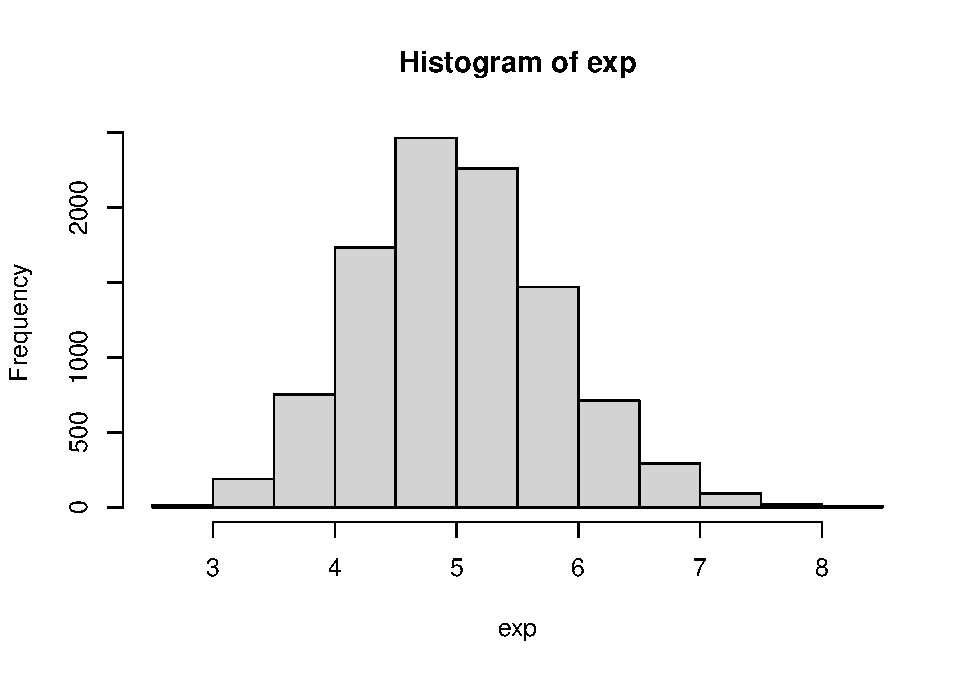
\includegraphics{CoursePrj1_files/figure-latex/simulation-1.pdf}

\begin{Shaded}
\begin{Highlighting}[]
\DecValTok{1}\OperatorTok{/}\FloatTok{0.2} \CommentTok{#theoretical mean}
\end{Highlighting}
\end{Shaded}

\begin{verbatim}
## [1] 5
\end{verbatim}

\begin{Shaded}
\begin{Highlighting}[]
\KeywordTok{mean}\NormalTok{(exp)}\CommentTok{#sample mean}
\end{Highlighting}
\end{Shaded}

\begin{verbatim}
## [1] 5.002809
\end{verbatim}

As could be seen theoretical and sample means are very close.

\hypertarget{variance-comparison}{%
\subsubsection{Variance comparison}\label{variance-comparison}}

Theoretical standard deviation: \(s=\frac{1/\lambda}{\sqrt{n}}\)

\begin{Shaded}
\begin{Highlighting}[]
\DecValTok{1}\OperatorTok{/}\FloatTok{0.2}\OperatorTok{/}\KeywordTok{sqrt}\NormalTok{(}\DecValTok{40}\NormalTok{) }\CommentTok{#theoretical sd}
\end{Highlighting}
\end{Shaded}

\begin{verbatim}
## [1] 0.7905694
\end{verbatim}

\begin{Shaded}
\begin{Highlighting}[]
\KeywordTok{sd}\NormalTok{(exp) }\CommentTok{#sample sd}
\end{Highlighting}
\end{Shaded}

\begin{verbatim}
## [1] 0.7928857
\end{verbatim}

Variance: \(\sigma=s^2\)

\begin{Shaded}
\begin{Highlighting}[]
\NormalTok{(}\DecValTok{1}\OperatorTok{/}\FloatTok{0.2}\OperatorTok{/}\KeywordTok{sqrt}\NormalTok{(}\DecValTok{40}\NormalTok{))}\OperatorTok{^}\DecValTok{2} \CommentTok{#theoretical variance}
\end{Highlighting}
\end{Shaded}

\begin{verbatim}
## [1] 0.625
\end{verbatim}

\begin{Shaded}
\begin{Highlighting}[]
\KeywordTok{var}\NormalTok{(exp) }\CommentTok{# sample variance}
\end{Highlighting}
\end{Shaded}

\begin{verbatim}
## [1] 0.6286678
\end{verbatim}

\hypertarget{show-that-distribution-is-approximately-normal}{%
\subsubsection{Show that distribution is approximately
normal}\label{show-that-distribution-is-approximately-normal}}

In a same manner we generate normal distribution with appropriate mean
and sd.

\begin{Shaded}
\begin{Highlighting}[]
\NormalTok{norm.sim=}\OtherTok{NULL}
\ControlFlowTok{for}\NormalTok{ (i }\ControlFlowTok{in} \DecValTok{1} \OperatorTok{:}\StringTok{ }\DecValTok{10000}\NormalTok{) norm.sim <-}\StringTok{ }\KeywordTok{c}\NormalTok{(norm.sim,}\KeywordTok{mean}\NormalTok{(}\KeywordTok{rnorm}\NormalTok{(}\DecValTok{40}\NormalTok{,}\DecValTok{5}\NormalTok{,}\DecValTok{5}\NormalTok{)))}
\end{Highlighting}
\end{Shaded}

I plot density plot for both distributions exponential and normal, as
could be seen visually the distribution of exponential simulation
follows that of normal.

\begin{Shaded}
\begin{Highlighting}[]
\NormalTok{exp.df <-}\StringTok{ }\KeywordTok{data.frame}\NormalTok{(exp) }\OperatorTok
\StringTok{  }\KeywordTok{mutate}\NormalTok{(}\DataTypeTok{label=}\StringTok{"exp"}\NormalTok{)}\OperatorTok
\StringTok{  }\KeywordTok{rename}\NormalTok{(}\DataTypeTok{value=}\StringTok{"exp"}\NormalTok{)}
\NormalTok{norm.df <-}\StringTok{ }\KeywordTok{data.frame}\NormalTok{(norm.sim)}\OperatorTok
\StringTok{  }\KeywordTok{mutate}\NormalTok{(}\DataTypeTok{label=}\StringTok{"norm"}\NormalTok{)}\OperatorTok
\StringTok{  }\KeywordTok{rename}\NormalTok{ (}\DataTypeTok{value=}\StringTok{"norm.sim"}\NormalTok{)}
\NormalTok{sim.df <-}\StringTok{ }\KeywordTok{rbind}\NormalTok{(exp.df,norm.df)}

\KeywordTok{ggplot}\NormalTok{(sim.df)}\OperatorTok{+}
\StringTok{  }\KeywordTok{geom_density}\NormalTok{(}\KeywordTok{aes}\NormalTok{(}\DataTypeTok{x=}\NormalTok{value,}\DataTypeTok{fill=}\NormalTok{label), }\DataTypeTok{alpha=}\NormalTok{.}\DecValTok{5}\NormalTok{)}\OperatorTok{+}
\StringTok{  }\KeywordTok{labs}\NormalTok{(}\DataTypeTok{title=}\StringTok{"Density plot for two simulated vectors"}\NormalTok{, }\DataTypeTok{x=}\StringTok{"values"}\NormalTok{)}\OperatorTok{+}
\StringTok{  }\KeywordTok{scale_fill_discrete}\NormalTok{(}\DataTypeTok{name=}\StringTok{"Legend"}\NormalTok{, }\DataTypeTok{labels=}\KeywordTok{c}\NormalTok{(}\StringTok{"Exponential"}\NormalTok{,}\StringTok{"Normal"}\NormalTok{))}
\end{Highlighting}
\end{Shaded}

\includegraphics{CoursePrj1_files/figure-latex/unnamed-chunk-4-1.pdf}

\end{document}
